% !TeX root = ../thesis.tex

\section{Test Suite Assessment}

\subsection{Coverage}
The most frequently used metric to measure the quantity and thoroughness of a test suite is the \emph{code coverage} or \emph{test coverage} \cite[p.~467]{8016712}. The test coverage indicates which fraction of the application code is hit by at least one test case in the test suite. Internally, a coverage framework calculates the coverage ratio by augmenting every application statement using binary instrumentation. A hook is inserted before and after every statement to detect which statements are executed by the test cases. Many different criteria exist to interpret these results and thus to express the fraction of covered code \cite{Myers:2011:AST:2161638}. The two most commonly used criteria are \emph{statement coverage} and \emph{branch coverage}.

\paragraph*{Statement coverage} Statement coverage expresses the fraction of statements that are executed by any test case in the test suite, over the total amount of statements in the code \cite{6588537}. Similarly, we can calculate the \emph{line coverage} as the fraction of covered code lines. Since one statement can span multiple lines and one line may also contain more than one statement, both of these criteria are intrinsically related. Statement coverage is heavily criticised in literature \cite[p.~37]{Myers:2011:AST:2161638} since it is possible to achieve a statement coverage percentage of $\SI{100}{\percent}$ on code of which we can prove it is malfunctioning. Consider \cref{lst:statement-coverage-fail}. If a test case would call the \texttt{example}-function twice with the arguments $\{a = 1, b = 2\}$ and $\{a = 5, b = 0\}$, then both test cases will pass and every statement will be covered, resulting in a statement coverage of $\SI{100}{\percent}$. However, suppose we would call the function with arguments $\{a = 0, b = 0\}$. The first argument matches the first condition of the branch but will trigger a \texttt{division-by-zero} error, even though the previous combination of arguments reported a complete statement coverage. This simple example was already sufficient to illustrate that statement coverage is not trustworthy. However, statement coverage may still prove useful for other purposes, such as detecting unreachable code which we may safely remove.

\begin{lstlisting}[caption=Irrelevant statement coverage in C.,label=lst:statement-coverage-fail,language=C]
int example(int a, int b) {
  if (a == 0 || b != 0) {
    return a / b;
  }
  
  return 0;
}
\end{lstlisting}

\paragraph*{Branch coverage} requires that the test cases traverse every branch of a conditional statement at least once  \cite[p.~37]{Myers:2011:AST:2161638}. For an \texttt{if}-statement, we require two test cases, one for every possible outcome of the condition (\texttt{true} or \texttt{false}). For a loop-statement, we require at least two test cases as well. One test case should never execute the loop, and the other test case should execute every iteration. Optionally, we can add additional test cases for specific iterations. Observe that, while this criterion is stronger than statement coverage, it will still not detect the bug in \Cref{lst:statement-coverage-fail}. In order to mitigate this, we can use \emph{multiple-condition coverage} \cite[p.~40]{Myers:2011:AST:2161638}. This criterion requires that for every conditional expression, every possible combination of subexpressions is evaluated at least once. If we apply this requirement to \Cref{lst:statement-coverage-fail}, the \texttt{if}-statement will only be covered if we test the following four cases.

\begin{itemize}
	\item $a = 0, b = 0$
	\item $a = 0, b \neq 0$
	\item $a \neq 0, b = 0$
	\item $a \neq 0, b \neq 0$
\end{itemize}

% komma voor ,and ? -> zoek regels op
\noindent It should be self-evident that achieving and maintaining a coverage percentage of $\SI{100}{\percent}$ at all times is critical. However, this does not necessarily imply that every line of code, every statement or every branch must be explicitly covered \cite{dein_2019}. Some parts of the code might be irrelevant or untestable, such as wrapper or delegation methods that only call a library function. All major programming languages have frameworks and libraries that enable the collection of coverage information during test execution, and each of these frameworks allows the exclusion parts of the code from the final coverage calculation. As of today, the most popular options are JaCoCo\footnote{\url{https://www.jacoco.org/jacoco/}} for Java, coverage.py\footnote{\url{https://github.com/nedbat/coveragepy}} for Python and simplecov\footnote{\url{https://github.com/colszowka/simplecov}} for Ruby. These frameworks report in-depth statistics on the covered code and indicate which parts require more extensive testing, as illustrated in \Cref{fig:coverage-statistics}.

\begin{figure}[!hbp]
	\subfloat[JaCoCo coverage report of \url{https://github.com/thepieterdc/dodona-api-java}.]{%
		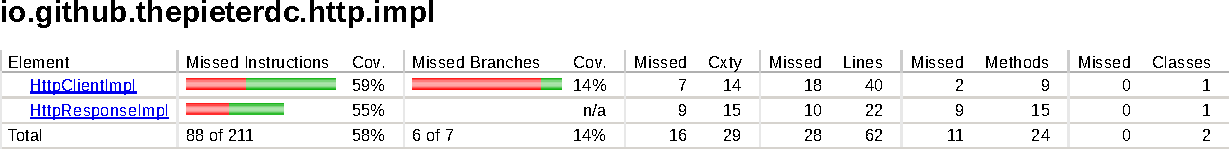
\includegraphics[width=\textwidth]{assets/images/coverage-jacoco.pdf}
	}
	\phantomcaption
\end{figure}
\begin{figure}[!ht]
	\ContinuedFloat
	\subfloat[coverage.py report of \url{https://github.com/codecov/example-python}.]{%
		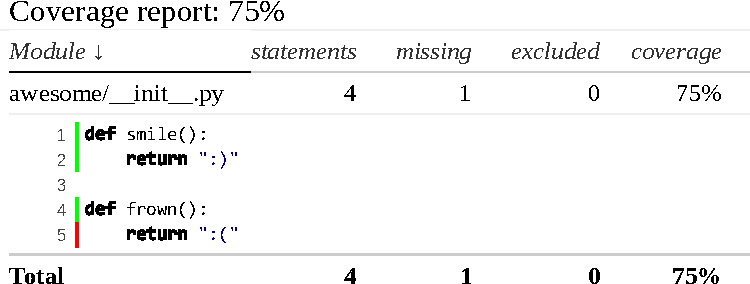
\includegraphics[width=\textwidth]{assets/images/coverage-coveragepy.pdf}
	}
	\phantomcaption
\end{figure}
\begin{figure}[!ht]
	\ContinuedFloat
	\centering
	\subfloat[simplecov report of \url{https://github.com/dodona-edu/dodona}.]{%
		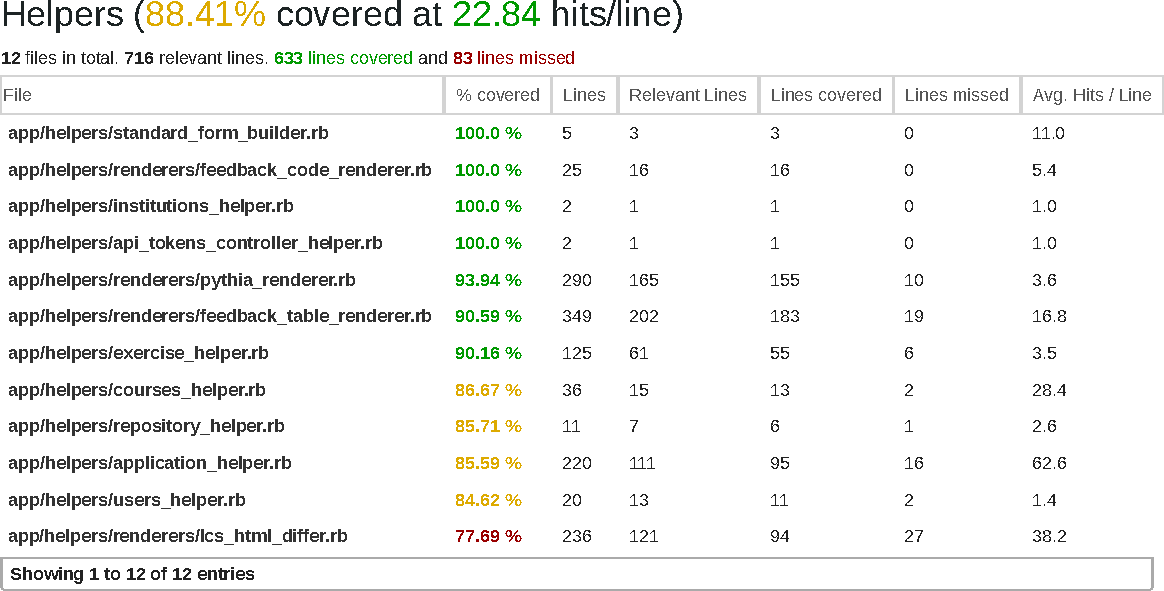
\includegraphics[width=\textwidth]{assets/images/coverage-simplecov.pdf}
	}
	\caption{Statistics from Code coverage frameworks.}
	\label{fig:coverage-statistics}
\end{figure}

\clearpage

% In the previous section. (section zelf heeft niets uitgelegd)
\subsection{Mutation testing}\label{sssec:mutation-testing}
The previous section has explained how we can identify which parts of the code require additional test cases. However, we cannot yet measure the quality and resilience of the test suite nor its ability to detect future failures. To accomplish this, we can employ \emph{mutation testing}. This technique creates several \emph{mutants} of the application under test. A mutant is a syntactically different instance of the source code. We can create a mutant by applying one or more \emph{mutation operators} to the original source code. These mutation operators attempt to simulate typical mistakes that developers tend to make, such as the introduction of off-by-one errors, removal of statements and the replacement of logical connectors \cite{Offutt2001}. The \emph{mutation order} refers to the amount of mutation operators that have been applied consecutively to an instance of the code. This order is traditionally rather low, as a result of the \emph{Competent Programmer Hypothesis}, which states that programmers develop programs which are near-correct \cite{5487526}.

\paragraph*{Creating and evaluating} the mutant versions of the code is a computationally expensive process which typically requires human intervention. As a result, very few software developers have managed to employ this technique in practice. \Cref{fig:mutation-testing} illustrates the process of applying mutation testing. The first step is to consider the original program $P$ and a set of test cases $TS$, to which we apply mutation operators to construct a broad set of mutants $P'$. Next, we evaluate every test case $t \in TS$ on the original program $P$ to determine the correct behaviour. Note that this step assumes that if the original source code passes the test cases, it is correct. 

% zoek of je sufficiently thorough of sufficient, thorough
This assumption will only be valid if the test suite contains sufficient thorough unit tests. If at least one of these test cases fails, we have found a bug which we must first resolve before continuing with the mutation analysis. When $P$ successfully passes every test case, we evaluate every test case for each of the mutants. A mutant $p'$ is said to be ``killed'' if its outcome is different from $P$ for at least one test case. Otherwise, we refer to the mutant as ``surviving''. After we have finished executing the test cases on every mutant, we analyse the set of surviving mutants. Every mutant that managed to survive implies a change in the source code that did not trigger any failure in the test cases. As a result, we need to introduce subsequent test cases until we have killed every mutant. However, it is also possible that the surviving mutants are functionally equivalent to $P$ and are, therefore, correct. Since the detection of program equivalence is an impossible problem, we need to verify this manually \cite{5487526, Offutt2001}. Finally, note that although we can use mutation testing to estimate the adequacy of the test suite, it is not flawless, as several mutation operators can cancel each other out \cite{evaluationoftestsuiteminimization}.

\clearpage

\noindent After every mutant has either been killed or marked equivalent to the original problem, we can calculate the \emph{mutation score} of the test suite using \Cref{eq:mutant-score}. In an adequate test suite, this score is equal to $\SI{1}{}$, which indicates that the test suite was able to detect every mutant instantly.

\begin{equation}\label{eq:mutant-score}
	\text{Mutant Score} = \frac{\text{killed mutants}}{\text{non-equivalent mutants}}
\end{equation}

\begin{figure}[h!]
	\centering
	\begin{tikzpicture}
\tikzset{
	edge/.style={->,> = Latex,semithick}
}

\def\xdiff{2.5cm}
\def\ydiff{2cm}

% Nodes.
\node[draw] (program)
{\begin{minipage}[c][1cm][c]{3.25cm}\centering Program $P$\end{minipage}};

\node[draw] (mutants) [right=\xdiff of program]
{\begin{minipage}[c][1cm][c]{3.25cm}\centering Mutants $P'$\end{minipage}};

\node[draw] (runtestsprogram) [below=\ydiff of mutants]
{\begin{minipage}[c][1cm]{3.25cm}\centering Run every test case $t$ on $P$\end{minipage}};

\node[draw] (testcases) [right=\xdiff of runtestsprogram]
{\begin{minipage}[c][1cm][c]{3.25cm}\centering Test Cases $TS$\end{minipage}};

\node[draw] (validatep) [below=\ydiff of runtestsprogram]
{\begin{minipage}[c][1cm][c]{3.25cm}\centering Validate correctness of $P$\end{minipage}};

\node[draw] (fixbugs) [left=\xdiff of validatep]
{\begin{minipage}[c][1cm][c]{3.25cm}\centering Fix bug in $P$\end{minipage}};

\node[draw] (runtestsmutants) [below=\ydiff of validatep]
{\begin{minipage}[c][1.25cm][c]{3.25cm}\centering Run every test case $t$ on every mutant $p'$\end{minipage}};

\node[draw] (aremutantsdead) [below=\ydiff of runtestsmutants]
{\begin{minipage}[c][1cm][c]{3.25cm}\centering All mutants killed?\end{minipage}};

\node[draw] (determineequivalence) [right=\xdiff of aremutantsdead]
{\begin{minipage}[c][1cm][c]{3.25cm}\centering Determine equivalence\end{minipage}};

\node[draw] (quit) [left=\xdiff of aremutantsdead]
{\begin{minipage}[c][1cm][c]{3.25cm}\centering Quit\end{minipage}};

\draw[edge] (program.east) -- (mutants.west)
node[midway,above]
{\begin{minipage}{2cm}\centering Apply mutation operators\end{minipage}};

\draw[edge] (mutants.south) -- (runtestsprogram.north);

\draw[edge] (runtestsprogram.south) -- (validatep.north);

\draw[edge] (validatep.west) -- (fixbugs.east)
node[midway,above] {Incorrect};

\draw[edge] (fixbugs.north) -- (program.south);

\draw[edge] (validatep.south) -- (runtestsmutants.north)
node[midway,left]
{\begin{minipage}[r]{2cm}\hfill Correct\end{minipage}};

\draw[edge] (runtestsmutants.south) -- (aremutantsdead.north);

\draw[edge] (aremutantsdead.west) -- (quit.east)
node[midway,above] {Yes};

\draw[edge] (aremutantsdead.east) -- (determineequivalence.west)
node[midway,above] {No};

\draw[edge] (determineequivalence.north) -- (testcases.south)
node[midway,right,rotate=90,anchor=north]
{Can add test cases to kill mutants};

\draw[edge] (testcases.west) -- (runtestsprogram.east);

\path (determineequivalence) edge [->,>=Latex,semithick,bend left=25] node [align=center,below]
{\begin{minipage}{7cm}\centering Every remaining mutant is functionally equivalent to $P$\end{minipage}} (quit);

\end{tikzpicture}

	\caption{Process of Mutation Testing (based on \cite{Offutt2001}).}
	\label{fig:mutation-testing}
\end{figure}